\chapter{Testovací scénáře a realizace pro VNF a NFV}

V předchozí kapitole byla popsána oblast virtualizace síťových funkcí a její architektura. Také byly popsány jednotlivé technologie, které budou v této kapitole použity pro vytvoření NFV frameworku, který bude následně využít k realizaci ukázkových VNF. Jak již bylo řečeno, tak pro každou VNF zde bude uveden příklad jejího použítí a jakým způsobem je možné vytvořit automatizované řešení pro VNF nad navrženým NFV frameworkem.

\section{Scénáře pro použití vybraných VNF}

Před somotnou implementací je nutné vysvětli, jakým způsobem budou VNF využívat uživatelé. Toto by mělo sloužit pro lepší pochopení daných příkladů a usnadnit realizaci jednotlivých VNF. Dále v této sekci budou postupně uvedeny jednotlivé scénáře pro všechna uvedené VNF v této práci. 

\subsection{Scénář LbaaS}

Jedním z často využívaných síťových funkcí je load balancing. Pokud chce uživatel v cloudu provozovat nějaký druh webové služby, která musí být vysoce dostupná nebo bude velice vytížená, tak bude ve většině případů potřebovat využít více než jeden server. Pro rozdělení zátěže mezi tyto servery by následně použil fyzický load balancer. Ten bude spravovat příchozí komunikaci a distribuovat ji mezi několika serverů. Tím bude zajištěna rozloha zátěže a zajištěn bezvýpadkový provoz.

Uvažujme tedy jednoduchý příklad, ve které bude uživatel chtít dva servery, na kterých poběží webová služba v HA. Pro tuto službu bude chtít využít cloudovou platformu s podporou LbaaS. Uživatel samozřejmě požaduje, aby se celá infrastruktura a nastavení webové aplikace proběhlo automaticky s co možná nejméně manuálními zásahy. Celý proces by se tedy v praxi měl skládat z výběru vhodného templatu, zadáním požadovaných vstupních parametrů (IP adresy, názvy instancí, atd.) a následné spuštění templatu, který vytvoří vše požadované. Obrázek č. \ref{fig:loadbalancer} zobrazuje požadovaný výstup tohoto procesu.

\begin{figure}[h]
\begin{centering}
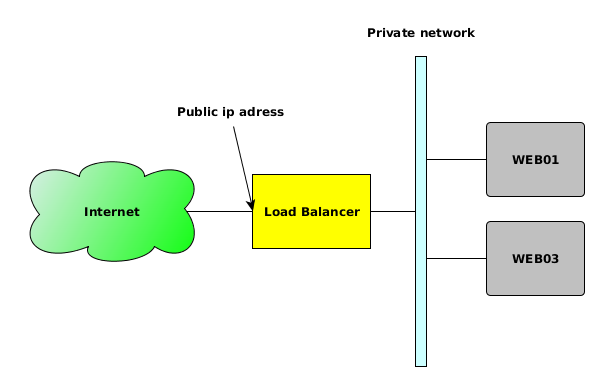
\includegraphics[scale=0.6]{images/LoadBalancer}
\par\end{centering}
\caption{Firewall as a Service\label{fig:loadbalancer}}
\end{figure}

Je tedy vidět, že VNF pro load balancing by měla být již integrovanou součástí návrhu cloudové aplikace, resp. návrhu cloudového templatu pro orchestraci. V případě HAproxy by toto neměl být problém, protože je to standartní součást OpenStacku a OpenContrailu. Mělo by tedy jít využít standarního heat templatu, ve kterém bude nadefinované vše potřebné pro Load Balancer. Otázkou je, zda bude možné využít stejný postup i případě AVI networks řešení.

\subsection{Scénář FwaaS}

Další z často využívaných síťových funkcí je firewall, resp. síťové funkce, které dokáží řídit a zabezpečovat síťový provoz mezi různými sítěmi. Zjednodušeně se dá říct, že slouží jako kontrolní bod, který definuje pravidla pro komunikaci mezi sítěmi, které od sebe odděluje.

Příkladů užití FwaaS v cloudovém prostředí existuje značné množství, protože uživatelé mohou mít různé požadavky na řízení datového provozu. Uvažujme však nejjednodušší příklad, kterým je překlad adres tzv. NAT. V tomto případě uživatel chce vytvořit virtuální instanci, která by měla mít konektivitu k externí síti, ale zároveň nechce, aby daná instance byla dostupná z této externí sítě. 

Otázkou zde je, jakým způsobem by měl být daný firewall nakonfigurován? Jak bylo popsáno kapitole \ref{sec:MANO}, tak existuje více možností. Konfigurace by mohla být doručena jako součást orchestračního templatu, např. v podobě skriptu, který by se provedl po spuštění firewall instance. Tento přístup však nemusí existovat podpora ze strany PfSense a Fortigatu. V tom případě bude muset být využita jiná metoda, pro kterou však ve většině případů musí být vyhrazený dedikovaný interface, určený právě management. Tento interface múže být využit i pro manuální zásahy do konfigurace. Obrázek č. \ref{fig:firewall} zobrazuje schématické zapojení pro FwaaS.

\begin{figure}[h]
\begin{centering}
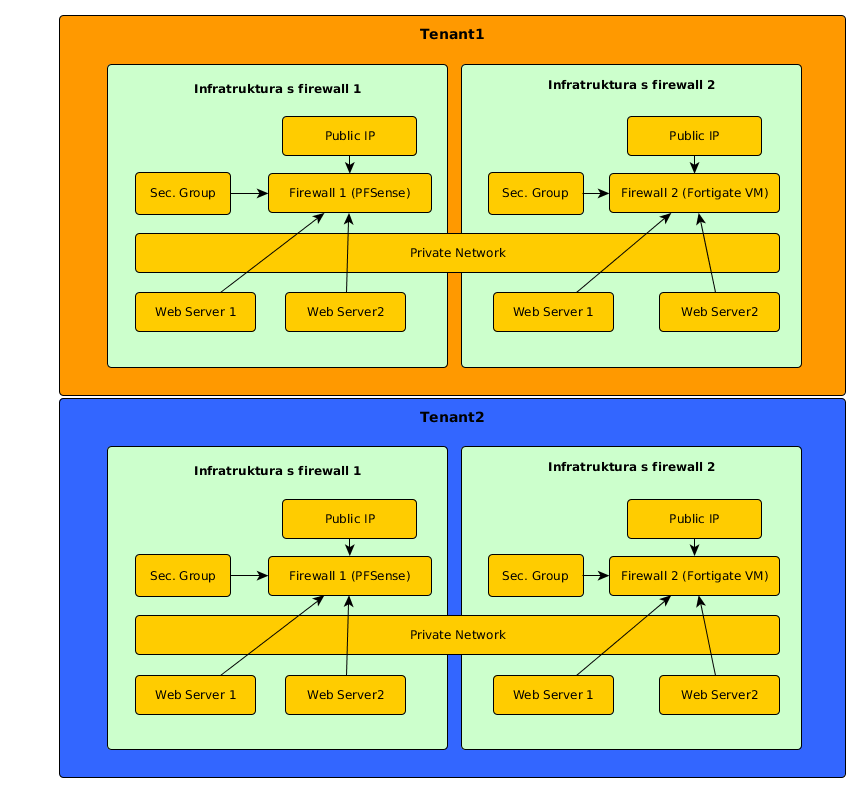
\includegraphics[scale=0.6]{images/firewall}
\par\end{centering}
\caption{Firewall as a Service\label{fig:firewall}}
\end{figure}


\section{Realizace VNF pro LbaaS} \label{sec:realizace_lbaas}

Zde již budou vysvětleny jednotlivé kroky související s realizací VNF pro LbaaS. Nejprve je ukázáno řešení s využitím HAproxy. Popsaný je zde obecný popis funkce haproxy, resp. LbaaS Neutronu a popis toho, jak byl využit pro tvorbu VNF. Po této ukázce následuje popis a vysvětlení realizace VNF související s platformou od AVI networks.

\subsection{HAproxy - Neutron HAproxy agent}

OpenStack Neutron ve své implementaci obsahuje službu LBaaS. Je to jedna z jeho pokročilou služeb, která umožňuje použít jeden soubor API k ovládání load balanceru od poskytovatelů třetích stran. Jedinou podmínkou je, aby toto API implementovali. Toto velice zjednodušuje uživatelům OpenStacku ovládání load balancerů a odpadá díky tomu nutnost seznamování se s implementací a konfigurací těchto různých řešení, která mohou být velmi specifická a odlišná. HAproxy je defaultní backend sloužící pro LbaaS pro OpenStack s využítím OpenContrailu jako SDN řešení. 

Load balancer se v Neutron LbaaS skládá ze základních 4 objektů, které jsou vzájemně provázány. Tyto objekty jsou:

\begin{itemize}
\item Pool - Obsahuje základní parametry pro load balancer. Jako je např. síťový rozsah, ve kterém budou webové servery či metodu pro distribuci zátěže (Round Robin, Least connection, atd.)
\item Virtuální IP (VIP) - ip adresa, na kterou přichází komunikace
\item Member - Je konkrétní virtuální instance, která je členem poolu např. webový server. Označení membera je pomocí jeho ip adresy.
\item Monitor - Periodicky kontroluje stav jednotlivých serverů a aplikací. Kontrola může být pomocí pingu či http a https dostupnosti.
\end{itemize}

Obrázek č. \ref{fig:NeutronLbaaS} zachycuje jednotlivé závislosti mezi těmito objekty.

\begin{figure}[h]
\begin{centering}
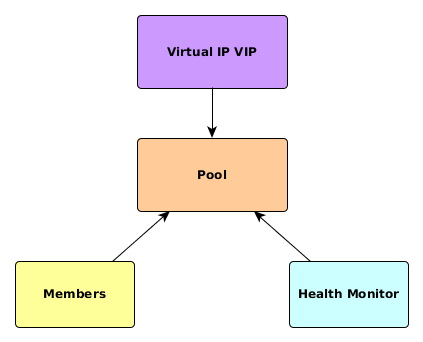
\includegraphics[scale=0.63]{images/NeutronLbaaS}
\par\end{centering}
\caption{Neutron LbaaS\label{fig:NeutronLbaaS}}
\end{figure}

Celý proces probíhá tak, že každý virtuální server, který je asociovaný s daným poolem z něj obdrží IP adresu. Když příjde na VIP nějaký dotaz na danou webovou aplikaci, tak je tento dotaz předán dál na jednu z těchto přiřazeným IP adres. Pokud nastane s aplikací či serverem nějaký problém, který zachytí monitor, tak load balancer ip adresu tohoto serveru přestane posílat komunikaci, dokud není vše zase v pořádku. 

Z výše uvedených informací vyplívá, že je nutné správně nadefinovat jednotlivé komponenty v heat templatu tak, abychom dosáhli požadovaného chování. Tím bude zajištěné správné a automatické řešení pro VNF.

\subsubsection{Heat template pro haproxy}

Celý heat template pro LbaaS s HAproxy v sobě obsahuje několik prostředků, které se po jeho spuštění pokusí heat engine vytvořit. Tvorba heat templatu vycházela z informací uvedených v dokumentaci \cite{HEAT}. Protože celý heat template je značně dlouhý, tak zde nebude ukazován celý jeho kód, ale pouze části týkájící se load balanceru. V případě zájmu lze celý template nalést v příloze. Template se tedy skládá z:

\begin{itemize}
\item Privátni síť - K této síti jsou připojeny obě webové instance, load balancer a router. Součástí je definice toho zdroje jsou je i subnet, který má dále paramentry týkající se DHCP ip adres.
\item 2 x web instance - jedná se o virtuální instance s operačním systémem Ubuntu 14.04. Po spuštění heat templatu se na tyto instance nainstaluje Apache server a vytvoří se index.html. Díky tomu je možné následně otestovat zda load balancer distubuje komunikaci mezi těmito dvěma servery.
\item router - toto je Neutron router implementují SNAT. V tomto příkladě je využívaný webovými servery pro konektivitu k Internetu. Toto je nutné pro nainstalování programu Apache na webové servery.
\item public síť - toto je veřejná síť, ze které je získána VIP pro load balancer. Na tuto VIP bude dále asociována floating ip. 
\item members - po vytvoření instancí je nutné jejich přidání do poolu jako membery. Pokud webová aplikace na serverch využívá jiný port než port 80, je možné ho zde změnit.

\begin{lstlisting}[caption=Healt monitor]
lb_pool_member_instance_01:
    type: OS::Neutron::PoolMember
    properties:
      address: { get_attr: [ instance_01 , first_address ] }
      admin_state_up: True
      pool_id: { get_resource: lb_pool }
      protocol_port: 80
      weight: 1
\end{lstlisting}

\item health monitoring - zdroj pro monitoring. Dle zvolených parametrů je vidět, že každých 5 sekund bude poslán ping na servery a bude se čekat 5 sekund na odpověď. Pokud nepříjde, tak load balancer usoudí, že je daný server není v pořádku a přestane na něj přeposílat komunikaci.

\begin{lstlisting}[caption=Healt monitor]
lb_ping_healt_monitor:
    type: OS::Neutron::HealthMonitor
    properties:
      admin_state_up: True
      delay: 5
      max_retries: 1
      timeout: 5
      type: PING
\end{lstlisting}

\item pool - jedná se o definování poolu pro load balancer. Na ukázce je vidět, že byla zvolena metoda Round Robin. Tato metoda byla zvolena kvůli co nejjednoduššímu testování tohoto templatu.

\begin{lstlisting}[caption=Healt monitor]
lb_pool:
    type: OS::Neutron::Pool
    properties:
      admin_state_up: True
      lb_method: ROUND_ROBIN
      name: { get_param: lb_name }
      protocol: HTTP
      monitors:
      - { get_resource: lb_ping_healt_monitor }
      subnet_id: { get_resource: private_subnet }
      vip:
        protocol_port: 80
        admin_state_up: True
        subnet: { get_resource: public_subnet }
\end{lstlisting}
\end{itemize}

Takto byl vytvořen heat template, který vytvoří LbaaS pomocí HAproxy. Nyní je nutné tento template otestovat, zda funguje správně.

\subsubsection{Testování heat templatu pro haproxy}

V reálném případě by si uživatel heat template vybral z katalogu. Avšak v rámci testovaní bude heat template spouštěn pomocí příkazu v terminálu:

\begin{lstlisting}
heat stack-create -f heat/templates/lbaas_template.hot -e heat/env/lbaas_env.env lbaas
\end{lstlisting}

Tento příkaz vytvoří všechny prostředky uvedené v templatu pro load balancing. Na obrázku č. \ref{fig:lbaas_topologie} je zobrazek screenshot vytvořené topologie z OpenStack dashboardu. Jsou zde vidět vytvořené servery a sítě. Není zde zobrazen load balancer, protože tato vizualizace tento prvek nezobrazuje. Lze ho nalézt v jiné části dashboardu, ale pro názornost bude rovnou otestováno jeho správné chování.

\begin{figure}[h]
\begin{centering}
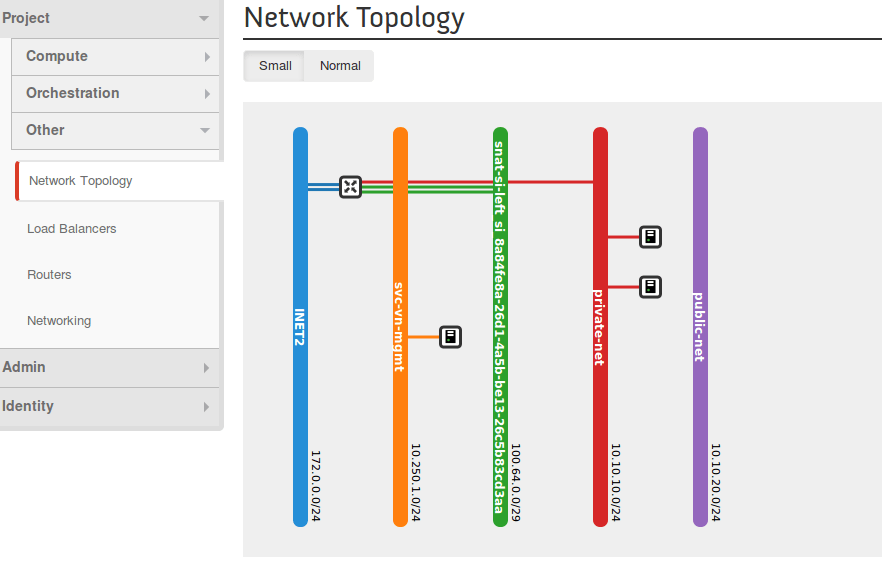
\includegraphics[scale=0.45]{images/lbaas_topologie}
\par\end{centering}
\caption{Vytvořená síťová topologie\label{fig:lbaas_topologie}}
\end{figure}

Otestování správného chování virtuálního load balanceru, lze provést opakovaným dotazem na právě vytvořené webové servery. Tím bude zároveň otestována jejich správná konfigurace. Pokud by totiž nevrátili správnou odpoveď je možné, že chyba může být i zde. 

Dotaz na webové servery byl proveden pomocí příkazu curl, kterému byla dána jako parametr public adresa load balanceru. Celý výstup toho testování znázorňuje obrázek č. \ref{fig:lbaas_testing}. 

\begin{figure}[h]
\begin{centering}
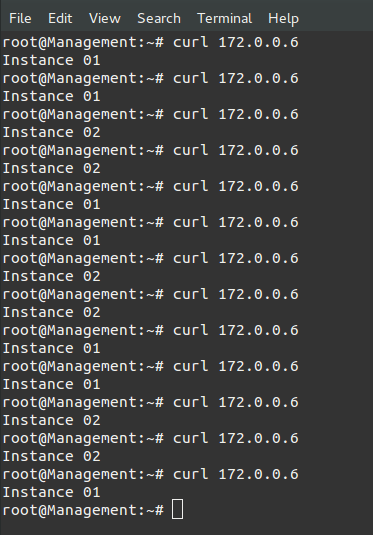
\includegraphics[scale=0.45]{images/lbaas_testing}
\par\end{centering}
\caption{Test konektivity a load balancingu\label{fig:lbaas_testing}}
\end{figure}

Po několika takovýchto dotazech na webové servery je vidět, že odpověď příchází střídavě od obou webových serverů. Probíhá mezi nimi tedy load balancing metodou round robin tak, jak bylo požadováno.

\subsection{AVI networks}

Druhým řešením pro LbaaS, které bude popsané a otestované v této práci, bude platforma od AVI networks. Narozdíl od HAproxy není tato platforma standarní součástí OpenStacku. Z tohoto důvodu musela být nejprve do testovacího prostředí nainstalována. 

Instalace spočívá ve vytvoření tenantu, ve kterém je nasledně vytvořena virtuální instance z image pro AVI Controller. Této instanci je následně nutné přidat IP adresu, aby k ní bylo možné přistoupit zkrze webový prohlížeč. Poté již následuje jednoduchá konfigurace, kde nutné správně nastavit připojení na keystone server. Tím je zajištěna integrace s OpenStackem. 

Po úspěšné instalaci vznikla v OpenStacku další služba, která umožňuje vytváření load balancerů ve všech tenantech. Vše funguje tak, že uživatel většinou přes AVI Controller dashboard, kde se přihlásí pomocí uživatele v keystonu, zvolí vytvoření virtální služby, kde vybere servery a nastaví požadované parametry. Na základě těchto udajů controller vytvoří tzv. Service Engine, který prování load balancing. Tento Service Engine vžak vznikne stále v tenantu určeném pro AVI networks, nikoliv v uživatelově tenantu. Obrázek č. \ref{fig:avi} znázorňuje toto řešení.

\begin{figure}[h]
\begin{centering}
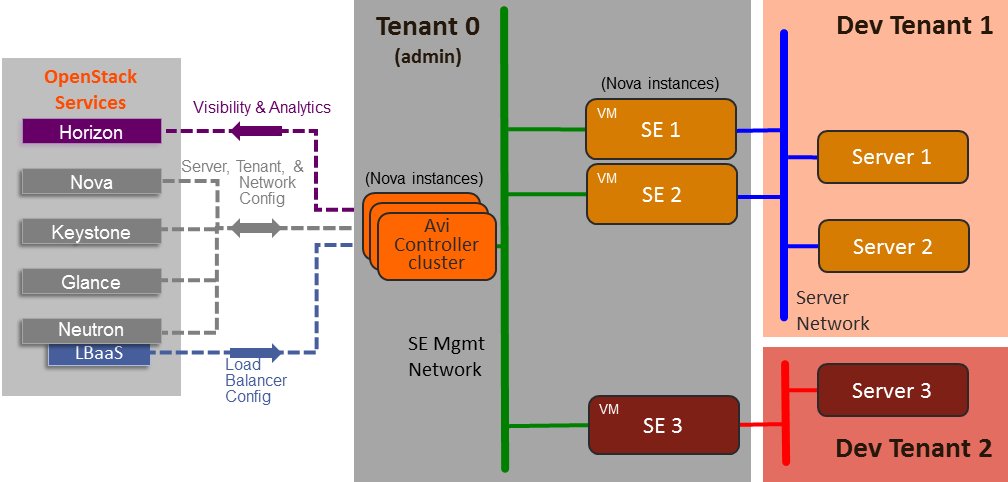
\includegraphics[scale=0.5]{images/avi}
\par\end{centering}
\caption{Znázornění funkce AVI networks LbaaS, převzato z \cite{avi_networks} \label{fig:avi}}
\end{figure}

Přestože vytváření a ovládání LbaaS zkrze dashboard bylo otestováno a funguje, tak je zde příliš manuálních kroků. Avšak při analýze tohoto produktu bylo zjištěno, že AVI networks nově také poskytuje podporu pro vytváření potřebných zdrojů i pomocí heatu. 

\subsubsection{Heat template pro AVI networks}

Pro tvorbu heat templatu pro AVI networks byl stejný template jako pro HAproxy. S tím rozdílem, že byly nahrazeny části týkající se load balanceru. Pro lepší čitelnost zde tedy nebudou uvedeny části, které jsou v obou templatech a budou zde popsány pouze části, které se liší. Jsou to tyto dvě části:

\begin{itemize}
\item AVI network pool - Obsahuje základní parametry pro load balancer. Je především definice serverů resp. jejich ip adresu, mezi keterými bude následně probíhat load balancing. Také je zde možná volba metody pro load balancing. Zde byla zvolena metoda round robin jako v předchozím příkladě. 

\begin{lstlisting}[caption=AVI networks pool]
pool:
  type: Avi::LBaaS::Pool
  properties:
    name: "testpool"
    default_server_port: 80
    health_monitor_uuids:
      - {get_resource: hm}
    lb_algorithm: LB_ALGORITHM_ROUND_ROBIN
    servers:
      - ip:
          addr: { get_attr: [myinstance1, first_address] }
          type: V4
        port: 80
      - ip:
          addr: { get_attr: [myinstance2, first_address] }
          type: V4
        port: 80
\end{lstlisting}

\item AVI virtual service - Zde je definovaná především veřejná ip adresa a port. Přes tyto údaje se následně bude přistupovat k serverů, resp. webové aplikaci.

\begin{lstlisting}[caption=AVI networks healt monitor]
  vs:
    type: Avi::LBaaS::VirtualService
    properties:
      name: "testvs"
      pool_uuid: {get_resource: pool}
      ip_address:
        addr: 10.10.32.100
        type: V4
      services:
        - port: 80
      application_profile_uuid: get_avi_uuid_by_name:System-Secure-HTTP
\end{lstlisting}


\item AVI network healt monitor - Poslední částí je healt monitor pro sledování stavu jednotlivých serverů. V ukázce je vidět nastavení jednotlivých časovačů a také protokolu http. Monitor sleduje http odpoveď od serveru a pokud dostane odpoveď začínající 2xx či 3xx, tak označí server/aplikaci jako v pořádku a bude na ni zasílat data.

\begin{lstlisting}[caption=AVI networks virtual service]
hm:
  type: Avi::LBaaS::HealthMonitor
  properties:
    name: "mytesthm"
    receive_timeout: 2
    failed_checks: 2
    successful_checks: 6
    send_interval: 2
    type: HEALTH_MONITOR_HTTP
    http_monitor:
      http_response_code:
        - HTTP_2XX
        - HTTP_3XX
      http_request: "GET / HTTP/1.0"
\end{lstlisting}

\end{itemize}

Takto by tedy měla být vytvořena automatizovaná VNF využívající platformu od firmy AVI networks. Nyní ji zbývá otestovat.

\subsubsection{Testování heat templatu pro AVI networks}

Při testování heat templatu pro AVI networks bylo očekáváno, že zde bude dosaženo stejného stavu jako při použití dashboardu. Bohužel po spuštění daného templatu nedošlo k vytvoření požadovaných resourců a jeho běh skončil errorem. Při dalším zkoumání bylo zjištěno, že v době psaní této práce je podpora heat ze strany AVI networks přiliš nová (přibližně měsíc) a není zde vše naprosto funkční. Z tohoto důvodu nemohl být tento heat template otestován. 

\section{Realizace VNF pro FwaaS}

V této sekci jsou vysvětleny jednotlivé kroky související s realizací VNF pro FwaaS. Oproti předchozímu příkladu zde není přímá integrace s OpenStackem. Z tohoto důvodu bylo navrhnuto tvochu odlišné řešení. Nejprve bude vytvořena virtuální infrastruktura pomocí heat templatu a tzv. Servisních instancí v OpenContrailu. Toto se nebude příliš od předchozího případu. Avšak poté bude samostatně řešen management resp. dodání potřebné konfigurace do vytvořené instance pro firewall. Tato konfigurace musí mít všechno potřebné, aby firewall vykonával funkci NAT, která byla zvolena jako ukázková VNF v této práci.

\subsection{Servisní instance v OpenContrailu}

V OpenContrailu je sice možnost využívat implementaci routeru s SNAT, která umožnuje instancím v privátních sítích konektivitu s externí sítí. Pokud však uživatel potřebuje využít pokročilejší funkce firewallu, tak je možné vytvořit servisní instanci, která bude sloužit jako VNF. V té může být použit libovolný požadovaný image firewallu uživatele.

Dle informací uvedených v \cite{opencontrail_web}, tak servisní instance v OpenContrailu je jednoduše virtuální stroj, který poskytuje danou VNF. Zároveň je však možné využívat Service Chainingu, který byl popsán v kapitole č. 2. Úplně nejjednodušším příkladem může být virtuální stroj s operačním systémem GNU/Linux, který může sloužit jako router mezi dvěma sítěmi. 

Pro vytvoření servisní instance je nejprve určit Servisní template, ze kterého má být tato instance vytvořena. Ten obsahuje její obecný předpis, který má tyto parametry:

\begin{itemize}
\item Název - Název je označení daného Servisního Templatu. Pomocí něho lze následně identifikovat daný template a spustit dle jeho parametrů Servisní instanci. 
\item Image - Je image, který má být použit pro vytvoření dané servisní instance. V našem případě se bude jednat o image, který obsahuje požadované síťové funkce. Tento image musí před tím než může být použit  nahrán do OpenStacku Glance.
\item Service Type - V OpenContrailu, prozatím existují dva typy. Jsou to Trafic Analyzer a Firewall.
\item Service Mode - Zde se určuje v jakém modu daný template bude nastaven. Jsou zde 3 možnosti. , .

  \begin{itemize}
  \item Transparent - v tomto případě se jedná o neroutovaný firewall, neboli L2 firewall.
  \item In-Network - poskytuje výchozí bránu a průchozí traffic je routovaný. Tento mode může být využit pro NAT, HTTP proxy, atd.
  \item In-Network-NAT - zde je situace podobná jako u In-Network, ale navracející traffic nemusí být routovaný zpět do zdrojové sítě.
  \end{itemize}

\item Typy síťových portů - Zde se určuje kolik portů bude daná instance, vytvořená pomocí tohoto templatu mít a jaká bude jejich role. Jsou zde možnosti Left, Right a Management. 
\end{itemize}

Po úspěšném vytvoření Servisního templatu je možné z něj vytvořit libovolný počet Servis Instancí. Ty běží jako klasické instance v OpenStacku. Jak tedy vyplývá z výše uvedených informací, tak existují dva druhy servisních instancí v OpenContrailu. 

První z nich je Analyzer. Ten slouží k analýze a zachytávání síťového trafficu. Image pro tento typ servisní instance obvykle obsahuje protokolový analyzér a paketový sniffer, jako je například oblíbený program Wireshark. Tato instance dostává traffic, který je posílán mezi dvěma sítěmi. Tento traffic vybírá OpenContrail podle nastaveného pravidla pro dané sítě. Podle těchto pravidel je vybrána jen část trafficu, která je následně dána k dispozici servisní instanci. Samotná servisní instance nijak nemanipuluje s trafficem a ani do něj žádný negeneruje. Jednoduše lze říci, že má nastavený síťový port v promiskuitním modu a pouze pozoruje traffic. Poté jen hlásí zachycené události uživateli čí jiným entitám v síti. Obrázek č. \ref{fig:service_instance_anal} znázorňuje tento typ servisní instance.

\begin{figure}[h]
\begin{centering}
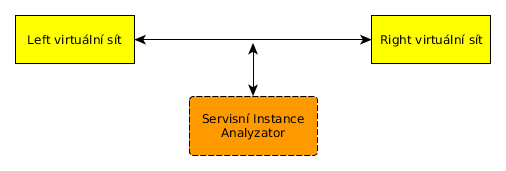
\includegraphics[scale=0.63]{images/service_instance_anal}
\par\end{centering}
\caption{Schéma zapojení servisní instance Analyzer\label{fig:service_instance_anal}}
\end{figure}

Je zde zřejmé, že pro účely této práce není Analyzer potřebný. Z tohoto důvodu bude dále uvažován pouze druhý typ servisní instance, kterým je Firewall. V tomto případě již servisní instance manipuluje s trafficem. Hlavní bodem, při vytváření servisní instance jako firewall, je přiřadit správné virtuální sítě k správným virtuálním síťovým portům. Servisní instance má obvykle dva síťové porty - left a right. Ty slouží pro propojení sítí do kterých jsou zapojeny. V některých případech je možné servisní instanci přidat i třetí síťový port, který slouží pro out-of-band management. Tento interface je vhodý předevím pro manuální management či pro management pomocí nějaké další entity.

\begin{figure}[h]
\begin{centering}
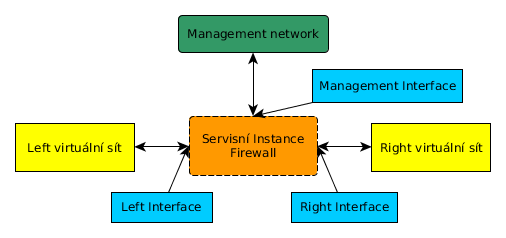
\includegraphics[scale=0.63]{images/service_instance}
\par\end{centering}
\caption{Schéma zapojení servisní instance\label{fig:service_instance}}
\end{figure}

Pro procházení síťové komunikace mezi sítěmi je nutné jí explicitně povolit v OpenContrailu pomocí tzv. Servisní policy. V tomto případě jich bude využito k vynucení toho, aby byla data posílána skrze servisní instanci.

Shrneme-li co vše je potřebné vytvořit pro FwaaS, tak je to servisní template, servisní instance z toho templatu a servisní policy. Toto vše lze naštěstí opět definovat v heat template, takže je možné toto všechno vytvořit automaticky jako v předchozím případě.

\subsection{Heat template pro FwaaS}

Heat template pro FwaaS byl navrhnut obdobně jako v případě LbaaS. Vzhledem k tomu, že template opět značně dlouhý, tak jeho kompletní verzi lze nalést v příloze. Tam lze také nalést enviroment file pro tento template. Zde bude uvedeno pouze to podstatné. Jeho součásti tedy jsou: 

\begin{itemize}

\item virtuální instance pro testování - Tato instance budou sloužit pro otestování správné funkčnosti VNF. Její hlavní činností bude generování dat v síti.

\item privátní síť - V této síti bude vytvořena instance pro testování. K této síti bude také připojen jeden z interfaců virtuální instance.

\item firewall template - Zde je ukázka pro vytvoření servisního tempaltu, který je použit v této práci. Většina parametrů by měla být dle názvu. Jediné co může být nejasné je paramenter "service interface type list". Do tohoto paramentru jsou v enviroment file vloženy názvy a pořadí jednotlivých interfaců. V našem případě používáme "management,right,left".

\begin{lstlisting}[caption=Servisní template]
service_template:
    type: OS::Contrail::ServiceTemplate
    properties:
      name: test-fw-template
      service_mode: in-network-nat
      service_type: firewall
      image_name: { get_param: template_image }
      service_scaling: True
      availability_zone_enable: True
      ordered_interfaces: { get_param: ordered_interfaces }
      flavor: { get_param: template_flavor }
      service_interface_type_list: { "Fn::Split" : [ ",", Ref: service_interface_type_list ] }
      shared_ip_list: { "Fn::Split" : [ ",", Ref: shared_ip_list ] }
      static_routes_list: { "Fn::Split" : [ ",", Ref: static_routes_list ] }
\end{lstlisting}

\item firewall instance - Tady je ukázán předpis pro tvorbu servisní instance. Je zde vidět, že instance bude vytvořena z již popsaného servisního templatu. Dále uveden seznam síťových interfaců společně s tím, kam se mají napojit. První se připojí do defaultní management sítě, kterou automaticky vytvoří OpenContrail, druhý do veřejné sítě a třetí do privátní.

\begin{lstlisting}[caption=Servisní instance]
service_instance:
  type: OS::Contrail::ServiceInstance
  depends_on: [private_subnet_1]
  properties:
    name: { get_param: private_instance_name }
    service_template: { get_resource:  service_template}
    availability_zone: { get_param: private_availability_zone}
    scale_out: 
        max_instances: 1
    interface_list: [
        {
            virtual_network: "auto"
        },
        {
            virtual_network: {get_param: public_net}
        },
        {
            virtual_network: {get_resource: private_net_1}
        }
    ]
\end{lstlisting}

\item contrail policy - Poslední co bylo nutné definovat pro FwaaS je servisní policy. Zde bylo pro jednoduchost povoleno vše z obou směrů pro servisnáí instanci. Tím bude jasné, že výsledný datový tok ovlivňuje pouze sdaná VNF.

\begin{lstlisting}[caption=Contrail network policy]
private_policy:
  type: OS::Contrail::NetworkPolicy
  depends_on: [ private_net_1, service_instance ]
  properties:
    name: { get_param: policy_name }
    entries:
      policy_rule: [
            { 
              "direction": "<>", 
              "protocol": "any", 
              "src_ports": [{"start_port": -1, "end_port": -1}],
              "dst_ports": [{"start_port": -1, "end_port": -1}],
              "dst_addresses": [{ "virtual_network": {get_param: public_net}}], 
              "action_list": {"apply_service": [{get_resource: service_instance}]}, 
              "src_addresses": [{ "virtual_network": {get_resource: private_net_1}}] 
            }, 
      ]
\end{lstlisting}
\end{itemize}

Tento template lze použít pro oba testované firewally. Jediné v čem se budou lišit jsou vstupní parametry, pro které budou dva oddělené enviroment soubory. Po spuštění daného templatu se vytvoří topologie, kterou znázorňuje obrázek č. \ref{fig:fwaas_topologie}. 

\begin{figure}[h]
\begin{centering}
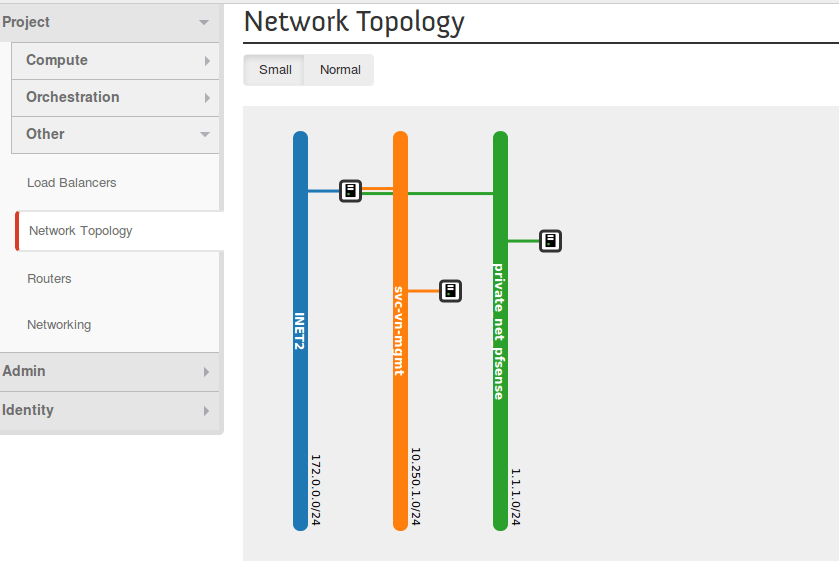
\includegraphics[scale=0.45]{images/fwaas_topologie}
\par\end{centering}
\caption{Síťová topologie\label{fig:fwaas_topologie}}
\end{figure}

Přestože výsledná síťová topologie je stejná pro PfSense i pro Fortigate VM, tak je dále nutné zajistit jejich správnou konfiguraci. Ta však dle bližším prozkoumání možností obou řešení bude značně odlišná. Proto již budou tyto informace uvedeny odděleně pro každý z obou firewallů. Je nutné ještě zmínit, že instance, ze které bude probíhat management, není součástí výše zmíněného templatu. Tato instance byla vytvořena samostatně. Je to z důvodu toho, že management nástoje by byly neústále smazávány při testování templatu a bylo by nutné nalést mechanismus, jak je vždy dostat zpět. 

\subsection{Management PfSense}\label{sub:interaction}

Pro management PfSense bylo oddzkoušeno několik možností. Je tomu tak, protože se ukázalo, že není úplně snadné proces konfigurace s PfSense elegantně vyřešit. 

Vzhledem k tomu, že PfSense je postavený na operačním systému FreeBSD, tak úplně prvním uvažovaným řešením měl být skript, který by byl součástí heat templatu. K tomu by však bylo nutné, aby jeho součástí byl tzv. cloud-init, který by tento skript z heat templatu převzal a provedl. Jeho nainstalování do PfSense bohužel bylo neúspěšné. 

Druhým přístupem bylo využítí konfiguračního managementu SaltStack. Informace o tomto nástroji, lze nalést zde \cite{salt}. Pro použití SaltStacku je nutné využít dvou jeho částí. První je tzv. Salt master. Ten obsahuje definici veškeré konfigurace pro infrastuktura, kterou spravuje. Ten je v námi uvažovaném případě nainstalovaný na management instanci a obsahuje potřebné informace pro správnou konfiguraci VNF. Druhou částí je tzv. Salt minion, který má za úkol přijímat příkazy od salt mastera a ty následně na cílové instanci definovaným způsobem vynutit. Avšak zde nastává problém, protože se opět nepodařilo správně nainstalovat salt miniona do PfSense instance.

Po předchozích neúspěších byl tedy zvolen nejjednodušší možný způsob. Tím je přednastavení požadované konfigurace do image s PfSense. Toto se ukázalo jako optimální řešení. Je tomu tak, protože tento image musel být stejně předem ručně vytvořen ze staženého instalačního souboru a následně nahrán do prostředí OpenStack, kde mohl být poté využíván. Předkonfigurování proběhlo přes PfSense dashboard, jehož ukázku ilustruje obrázek č. \ref{fig:nat}

\begin{figure}[h]
\begin{centering}
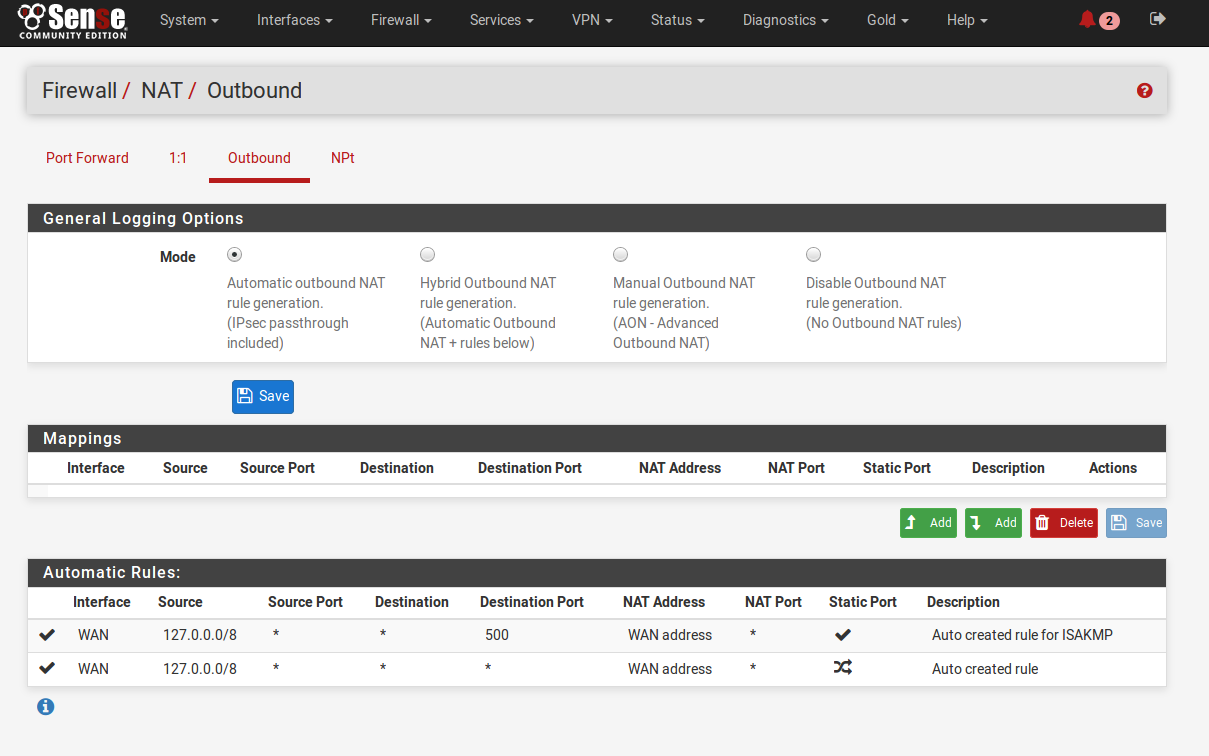
\includegraphics[scale=0.38]{images/nat}
\par\end{centering}
\caption{Konfigurace NAT v PfSense dashboardu\label{fig:nat}}
\end{figure}

Vše muselo být uspůsobeno tak, aby image byl co nejvíce generický. To znamená, že na všech interfacech bylo nastaveno dhcp, protože uživatel může zvolit naprosto jiné ip rozsahy než jsou používány v této práci. To samé platí pro pravidla, které PfSense využívá pro NAT. Ty museli počítat s tím, že na interfacech budou různé ip adresy, takže se v nich nesměla konkrétní ip adresa vyskytovat. Toho bylo dosaženo tak, že v pravidle pro NAT byla ip adresa resp. LAN subnet, který by je jinak specificky definovaný, byl nahrazen čtyřmi nulami (0.0.0.0). Tak bylo dosaženo dosaženo správného překladu adres, bez ohledu na přidělené ip adresy z OpenContrailu.

Toto řešení muselo být samozřejmě řádně otestováno. Test proběhl pomocí příkazu ping z testovací instance. Jak je vidět na obrázku č. \ref{fig:test_pfsense}, tak konektivita do externí sítě funguje.

\begin{figure}[h]
\begin{centering}
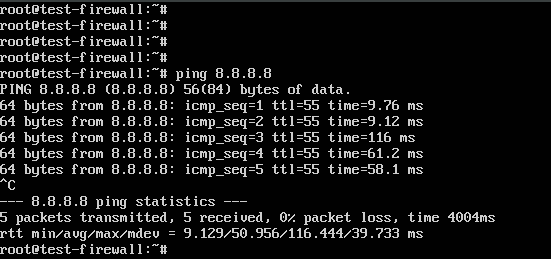
\includegraphics[scale=0.5]{images/test_pfsense}
\par\end{centering}
\caption{Test konectivity zkrze PfSense\label{fig:test_pfsense}}
\end{figure}

\subsection{Management Fortigate VM}

Management Fortigate VM probíhal obdobně jako u PfSense. Nejprve proběhlo hledání možností konfigurace zkrze skript v heat templatu. Zde však chybí jakákoli podpora doinstalace sofwaru třetích stran, takže opět nemohl být použit cloud-init. Další hledání však objevilo, že Fortigate VM poskytuje API, které může být využito pro jeho management. K tomu bylo využito python knihovny pro toto API a dokumentace \cite{pyfg}.


\begin{lstlisting}[caption=Fortigate konfigurace pro interface]
config system interface
edit port1
set type physical
set vdom root
set mode dhcp
set defaultgw disable
set allowaccess ssh ping http https
end
\end{lstlisting}

\begin{lstlisting}[caption=Skript pro nahrání konfigurace interfaců]
from pyFG import FortiOS
import sys
if __name__ == '__main__':
    f = open('fortios_intf.txt', 'r')
    candidate = f.read()
    f.close()
    d = FortiOS('fortigate', username="admin", password="fortigate")#, vdom='test_vdom')
    d.open()
    d.load_config('system interface', empty_candidate=True)
    d.load_config(config_text=candidate, in_candidate=True)
    config_changes = d.compare_config()
    d.commit(config_changes)
    d.close()
\end{lstlisting}

\begin{lstlisting}[caption=Fortigate konfigurace pro NAT]
config firewall policy
edit 1
set srcintf port3
set dstintf port2
set srcaddr all
set dstaddr all
set action accept
set schedule always
set service ALL
set logtraffic all
set nat enable
end
\end{lstlisting}


//Python API = skript
// => Salt module 


\section{Shrnutí získaných poznatků}